
\documentclass{report}
\usepackage[T1]{fontenc} % Fontes T1
\usepackage[utf8]{inputenc} % Input UTF8
\usepackage[backend=biber, style=ieee]{biblatex} % para usar bibliografia
\usepackage{csquotes}
\usepackage[portuguese]{babel} %Usar língua portuguesa
\usepackage{blindtext} % Gerar texto automaticamente
\usepackage[printonlyused]{acronym}
\usepackage{hyperref} % para autoref
\usepackage{graphicx}
\usepackage{indentfirst}

\bibliography{bibliografia}


\begin{document}
\def\titulo{Trabalho Cibersegurança}
\def\data{19 de dezembro de 2021}
\def\autores{Miguel Reis, Henrique Coelho}
\def\autorescontactos{(108545) mreis@ua.pt, (108342) hcoelho@ua.pt}
\def\versao{1}
\def\departamento{Departamento de Eletrónica, Telecomunicações, e Informática}
\def\empresa{Universidade de Aveiro}
\def\logotipo{ua.pdf}
\def\projeto{https://code.ua.pt/projects/trabalho-ciberseguranca}

%
%%%%%% CAPA %%%%%%
%
\begin{titlepage}

\begin{center}
%
\vspace*{50mm}
%
{\Huge \textbf{\titulo}}\\ 
%
\vspace{10mm}
%
{\Large {\empresa}}\\
%
\vspace{10mm}
%
{\LARGE \autores}\\ 
%
\vspace{20mm}
%
\begin{figure}[h]
\center
\includegraphics{\logotipo}
\end{figure}
%
\vspace{30mm}
\end{center}
%
\begin{flushright}
\versao
\end{flushright}
\end{titlepage}

%%  Página de Título %%
\title{%
{\Huge\textbf{\titulo}}\\
\vspace{5mm}
{\Large \departamento\\ \empresa}
}
%
\author{%
    \autores \\
    \autorescontactos\\
\projeto}

%
\date{\data}
%
\maketitle

\pagenumbering{roman}

%%%%%% RESUMO %%%%%%
\begin{abstract}
\vspace{2mm}
Neste trabalho iremos falar sobre a Cibersegurança, dando a conhecer o que é,como funciona, quais os seus principais domínios e ameaças e tabém dar a conhecer um pouco de como podemos melhorar a nossa cibersegurança, quer seja na vida pessoal ou profissional.

\vspace{4mm}
Iremos abordar a segurança das infraestruturas críticas e que devido ao seu grande impacto para a sociedade, uma falha numa dada infraestrutura/setor pode abranger muitas outras, devido às ligações entre elas(pois muitas dependem de outras) e o que o governo e outras organizações fizeram para evitar tais catástrofes.\\

\vspace{4mm}
Abordaremos também a importância da segurança de redes e como garantir a sua segurança. Além disso, também iremos falar das tarefas que introduzem um ciclo de vida de desenvolvimento de software seguro na segurança de um aplicativo (AppSec).\\

\vspace{4mm}
 Vamos mencionar também a importância da segurança em cloud e qual a sua diferença perante as outras redes e também enunciaremos a importância das empresas  ensinarem os seus trabalhadores a defenderem-se de certas ameaças, principalmente o phishing, uma técnica muito popular que espalha ransomware, para acrescentar à ideia da importâcia de ensinar para uma boa segurança, enumeramos uma serie de ações a ter de forma a melhorar a nossa cibersegurança.\\

\vspace{4mm}
Por fim, apresentaremos certas dicas para que um utilizador saiba que está a ser vítima de cibercriminosos, e enunciareremos algumas ações do que devemos imediatamente fazer após essa grande ameaça. 
\end{abstract}

%%%%%% Agradecimentos %%%%%%
% Segundo glisc deveria aparecer após conclusão...
\renewcommand{\abstractname}{Agradecimentos}
\begin{abstract}
Gostaríamos de agradecer a: 

\begin{description}
	\item[Professor António Manuel Adrego da Rocha ], pela orientação no trabalho e constante ajuda no esclarecimento de dúvidas acerca do trabalho de aprofundamento, sem o qual não conseguiríamos ter feito este trabalho.
	\item[\ac{ua}], pela cedência da bilbioteca e salas nas quais nos pudemos juntar de forma a realizar o trabalho.
	\end{description}
	
\end{abstract}


\tableofcontents
% \listoftables     % descomentar se necessário
% \listoffigures    % descomentar se necessário


%%%%%%%%%%%%%%%%%%%%%%%%%%%%%%%
\clearpage
\pagenumbering{arabic}

%%%%%%%%%%%%%%%%%%%%%%%%%%%%%%%%
\chapter{Introdução}
\label{chap.introducao}
A cibersegurança tem-se tornado um tema cada vez mais importante nas nossas vidas, a evolução da tecnologia faz com que cada vez estejamos mais dependentes dela e para garantir que temos a nossa informação segura. Decidimos avançar com este tema, pois é algo que consideramos bastante útil e interessante para dar a conhecer de forma a que possamos aproveitar ao maximo as tecnologias e fora de perigo.\\

Este documento está dividido em quatro capítulos.\\
Depois desta introdução,
no \autoref{chap.DefiniçaoCibersegurança} é introduzido noções gerais da cibersegurança.\\
No \autoref{chap.dominios} são apresentados os principais domínios em que a cibersegurança atua.\\
Finalmente, no \autoref{chap.conclusao} são apresentadas
as conclusões do trabalho.

\chapter{O que é a cibersegurança?}
\cite{DefCyber}
\cite{cisco}
\label{chap.DefiniçaoCibersegurança}
A cibersegurança tem-se tornado um tema cada vez mais importante nas nossas vidas, a evolução da tecnologia faz com que cada vez estejamos mais dependentes dela e para garantir que temos a nossa informação segura. Decidimos avançar com este tema, pois é algo que consideramos bastante útil e interessante para dar a conhecer de forma a que possamos aproveitar ao maximo as tecnologias e fora de perigo.
\section{Qual a sua importância?}
\cite{techtarget}
O custo das falhas da cibersegurança é uma das principais razões pela qual a cibersegurança é tão importante, não só o custo que uma falha pode significar na empresa como um simples ficheiro corrompido que pode significar enormes perdas para a empresa, mas também a ideia de a informação confidencial da empresa e dos seus clientes ser acedida por atacantes com intenções maliciosas podia completamente destruir uma empresa. De forma a combater estas falhas de segurança foram ainda criadas regras que implicam multas enormes para organizações que sofram falhas na sua cibersegurança, tornando assim cada vez mais uma aposta neste tema.\\
Porém, os ciberataques estão cada vez mais avançados e por isso temos nós também que evoluir de forma a evitar estes ataques, e sendo o cibercrime cada vez mais um grande negócio lucrativo vai atraindo inúmeros hackers que pretendem lucrar com o prejuízo e trabalho de outros. Por isso é importante investir na cibersegurança e garantir boas práticas no que toca à proteção dos nossos dispositivos.\\
\clearpage
\cite{wiki}

\maketitle\textbf{{Ciberataques comuns:}}\\
\begin{description}
    \item[Backdoors]-As backdoors permitem acesso remote a computadores ou sistemas sem o conhecimento do utilizador.
    \item[Formjacking]- É o processo de inserir código JavaScript malicioso em formulários de pagamentos online para retirar informações sobre os detalhes dos cartões de crédito dos clientes.
    \item[CryptoJacking]-Consiste na instalação maliciosa de mineradores de criptomoedas (“cryptomining software”). Este software danifica ilegalmente o poder de processamento do utilizador sendo este prejudicial para o computador do utilizador.
    \item [DDoS attacks]- Ataques \ac{DDoS} tentam romper o normal tráfico da web e atingir sites da web, servidores ou redes inundando os sistemas de modo a que fiquem offline, inundando esses sistemas com inúmeros pedidos de acesso até chegar ao ponto de o servidor não aguentar tantos pedidos e cair.
    \item [DNS poisoning attacks]- Ataques \ac{DNS}  comprometem o DNS de forma a redirecionar a sites maliciosos criados de forma a obter informações sobre o utilizador.
    \item [Injeção de Malware]-O malware é um termo usado para identificar ficheiros ou programas cuja intenção é danificar ou corromper o dispositivo.Existem diversos tipos de malware:
    \begin{enumerate}
    	\item Botnet Software-Consiste em software criado de forma a infetar um grande número de dipositivos conectados à Internet, cada um usando pouca percentagem do seu poder de processamento. Isto torna difícil a deteção deste tipo de malware mesmo que o ataque esteja a decorrer nesse momento.
    	\item Ransomware attacks- Este tipo de malware encripta a informação das vitimas de forma a que o hacker mais tarde possa pedir um pagamento para que a vitima possa ter novamente acesso a essa informação. Muitas vezes isto acontece e após o pagamento a informação não é devolvida mas sim novamente vendida na chamada “Dark Web”.
    	\item RATs (Remote-access Trojans)-  É um tipo de malware que instala as anteriormente referidas backdoors nos sistemas de forma a dar acesso remoto ou administrativo a utilizadores não autorizados.
    	\item Rootkits and Bootkits- Os Rootkits contêm diversos softwares maliciosos, funciona basicamente como um pack adquirível que dá aos hackers as ferramentas para atingir remotamente dispositivos.
Um Bootkit é basicamente um Rootkit mas que funciona antes do Sistema Operativo.
		\item Spyware- É uma forma de malware utilizada para acedar ilegalmente à atividade do computador e recolher informação pessoal.
    	\item Trojan- Um Trojan (inspirado na famosa história do Cavalo de Tróia) consegue camuflar-se como um software legítimo enquanto executa atividade maliciosa no dispositivo.
    	\item Viruses and worms- Um virus é uma parte de código malicioso instalada sem o conhecimento do utilizador. Os vírus conseguem assim replicar-se e espalhar-se por outros dispositivos agregados ao original. Estes vírus normalmente vêm a partir de trojans que o utilizador não consegue identificar como maliciosos
As worms são como os vírus, porém sem a necessidade de se anexarem a outos programas para se replicarem
    \end{enumerate}
      
\end{description}
\section{Como os cibercriminosos atuam?}
	Os cibercriminosos, também conhecido como hackers têm como principal objetivo aceder aos nossos dispositivos de forma a lucrar com isso. Para poderem aceder aos dispositivos, estes aproveitam-se das vulnerabilidades dos sistemas que usamos.\\
	As vulnerabilidades dos sistemas são as falhas de segurança a partir das quais os hackers atuam.
Existem várias vulnerabilidades conhecidas e disponíveis online para ser possível um melhoramento da segurança por parte dos profissionais, porém estas também são aproveitadas pelos hackers.\\
Tudo o que é necessário para que um criminoso explore estas vulnerabilidades são os Rootkits(referencia) e um simples tutorial online. Sem ser necessário nenhum conhecimento de programação.
Apesar dos ataques em maior escala serem mais trabalhosos todos têm por base a vulnerabilidade dos sistemas.

\chapter{Domínios da Cibersegurança}
\label{chap.dominios}
\cite{IBM}
Os principais domínios que temos de ter em atenção quando falamos sobre cibersegurança são os segunites.



\section{Critical Infrastructure Security}
\cite{CIP}
\cite{EPCIP}
\cite{cisa}
\normalsize{Critical infrastructure security (\ac{CIP}) é um conceito para a preparação e resposta a acidentes graves que envolvam uma região ou nação. As infraestruturas críticas estão relacionadas com a rede elétrica, a rede de transportes e os sistemas de informação e comunicação. Qualquer dano/destruição a estas infraestruturas, trará consequências negativas para a segurança e bem-estar da população de uma determinada nação/região. 
Para evitar tais consequências, os \ac{EUA}, para garantir a segurança das suas infraestruturas críticas, em maio de 1998, o presidente Bill Clinton criou uma diretiva, que foi atualizada mais tarde pelo presidente Bush, para não só a segurança, mas também para a identificação e priorização das infraestruturas críticas. Além dos \ac{EUA}, o Conselho Europeu, em 2004, criou o \ac{EPCIP}, um programa para identificar e proteger infraestruturas críticas, caso aconteça alguma falha pode afetar um país onde está hospedado como também um estado-membro europeu. Todos os estados-membros foram obrigados a adotar a \ac{EPCIP}.

A infraestrutura envolve vários setores, relativamente a banca de finanças, transporte, energia, informação e comunicações, agências de aplicação da lei, obras públicas, serviços federais e municipais, serviços de emergência, corpo de bombeiros, sendo incluído ainda mais setores em 2003 nomeadamente a agricultura e alimentos e, por fim, monumentos e ícones nacionais. Cada um destes setores, nos EUA, têm um departamento específico para coordenar a sua proteção. 

	Apesar da possibilidade de interligações entre setores, de modo a criar uma economia e um país mais eficiente e embora mais forte, pode trazer várias consequências. Quando vários setores estão interligados, por exemplo, a maioria dos setores citados no parágrafo anterior, alguns destes estão conectados ao setor de informação e comunicação, e um ataque terrorista a este campo/setor não afetará só o próprio, como também os outros ‘dependentes’ do mesmo, causando um efeito cascata. Pois, o setor de informação e comunicação trouxe vários aspetos positivos a vários setores dos \ac{EUA}, como também a reformular alguns processos, ficando mais orientados para o software. 

Como a infraestrutura se tornou um importante aspeto da salvação nacional, os terroristas conseguem fazer grandes quantidades de dinheiro ao atacando elementos da mesma. Isto deve-se ao simples facto de que ao desativar uma infraestrutura a defesa dessa nação irá diminuir, como também a confiança do público e a força económica. Além disto, ataques bem escolhidos podem ser menos gravosos do que a guerra tradicional, por causa da interdependência dos elementos da infraestrutura. Isto é, com o ataque, os terroristas podem pedir uma quantidade de dinheiro ao país sofredor, e caso este aceite a proposta, os terroristas se retiram.}
	
\begin{figure}[hp]
    \center 
    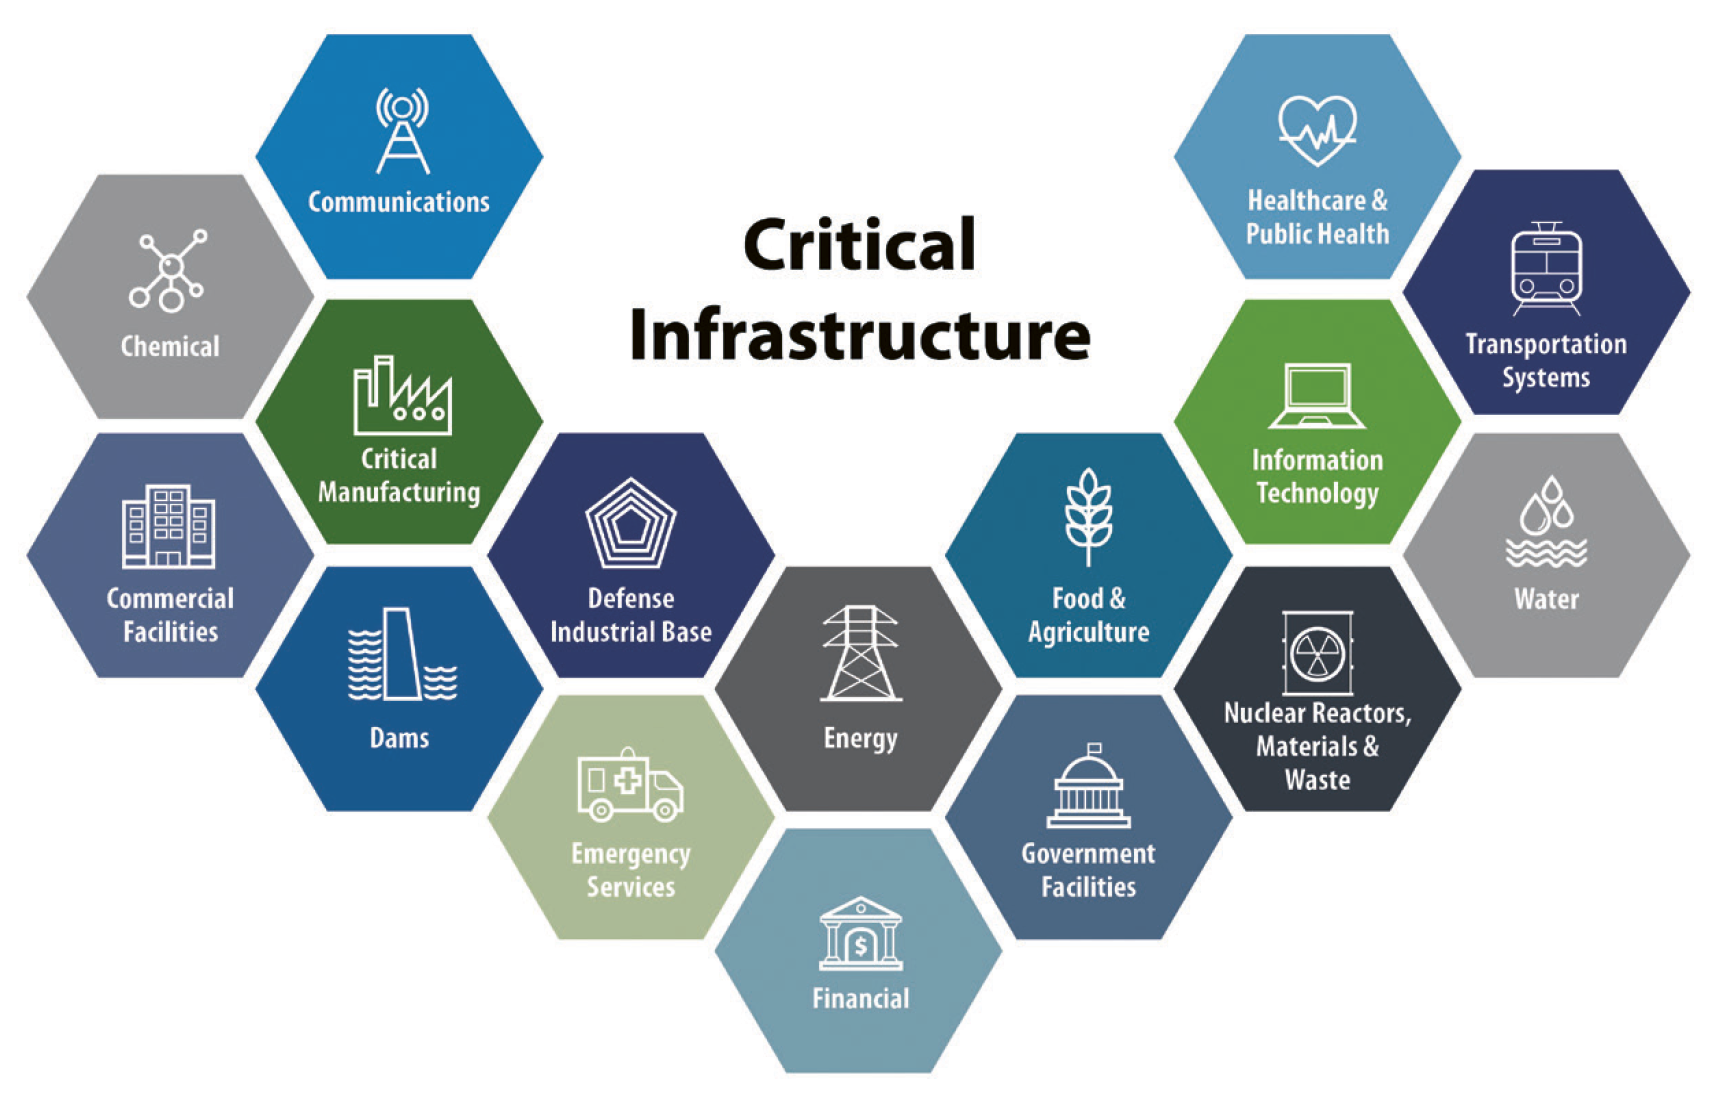
\includegraphics[height=200pt]{Figura1}
    \caption{Critical Infrastructure (SECTORS)}
    \label{fig:Figura1logo.1}
\end{figure}
\clearpage


\section{Network Security}
\cite{forcepoint}
\normalsize{Network security ou segurança de redes é um termo que serve para designar as tecnologias, dispositivos e processos que servem para garantir a integridade, confidencialidade e acessibilidade das redes de computadores e dados quer seja através de hardware ou software. Qualquer organização, independentemente do seu tamanho ou infraestrutura necessita de um bom grau de segurança na sua base de forma a proteger os seus interesses e clientes.
Existem vários níveis de segurança a considerar ao falar de segurança de redes. Os ataques podem acontecer a qualquer nível, por isso é importante ter uma boa segurança de hardware e software e boas políticas de privacidade.
Vamos falar sobre as diferentes maneiras de garantir uma boa segurança na nossa rede.
O controlo de acessos à rede (Network Access Control) é a prática de garantir que os atacantes não conseguem infiltrar-se na rede, isto é possível controlando todos os dispositivos e pessoas com acesso à rede e apenas conceder acesso aos maiores níveis de administração da rede a utilizadores específicos.
Outra forma de evitar ataques a nossa rede seria com softwares Antivírus e Antimalware, que protegem a organização de um a grande variedade de softwares maliciosos e vírus conhecidos. Isto é uma importante prática pois não só nos protege de riscos já conhecidos, mas estando em constante atualização garante que temos sempre a mais recente proteção ativa.
Todas as redes contêm uma proteção Firewall, que como o nome sugere é uma barreira que separa a nossa rede interna de outras redes exteriores não confiáveis.
Considerando que é preciso um constante acesso à nossa rede, existe uma maneira de garantir que a nossa transferência de ficheiros e dados é segura quando não nos encontramos a trabalhar na rede mas sim nos computadores pessoais, isto são as \ac{VPN} (Virtual Privacy Network) que criam uma conexão à nossa rede através de um ponto ou site de forma a que a comunicação entre o dispositivo usado e a rede seja encriptada e segura.
A segurança de redes deveria ser considerada com alta importância quer para uma organização ou até mesmo para o simples utilizador. Pois é nela que muitas vezes habita toda a nossa informação mais importante, à qual não queremos perder o acesso nem que vá parar às mãos erradas.}
\clearpage

\section{Application Security}
\cite{wiki2}
\cite{vmware}
A segurança do aplicativo (AppSec) inclui todas as tarefas que introduzem um ciclo de vida de desenvolvimento de software seguro para as esquipes de desenvolvimento. Tem como objetivo final aprimorar a segurança, localizar, corrigir e prevenir problemas de segurança nos aplicativos. 

Para aumentar a segurança de um aplicativo, são efetuados vários tipos de abordagens nomeadamente: 
\begin{itemize}
   \vspace{5mm} \item   \textbf{Revisão de design - }á medida que se avança no processo de desenvolvimento o custo de corrigir uma falha aumenta, portanto, de certeza que vale mais a pena fazer revisões á medida que se realiza a aplicação para descobrir erros mais cedo, corrigindo-os e evitado menos custos. Logo, fazer várias revisões de design são uma boa ‘política’;
    \vspace{5mm}\item   \textbf{Revisão de segurança da caixa branca ou revisão de código - }é uma atividade para melhorar a qualidade do software, para tal, uma ou mais pessoas reúnam-se para analisar um dado programa (lendo partes do seu código-fonte), de modo a atingir vários objetivos como melhorar a qualidade do código, encontrar defeitos, aprendizagem de conhecimento, aumentar o senso de responsabilidade mútua, encontrar melhores soluções e até mesmo em conformidade com as diretrizes de QA, padrões \ac{ISO/IEC}, principalmente para software de tráfico rodoviário/aéreo/náutico, devido de estarem em ‘jogo’ vidas, ou dano grave ao equipamento. Mas atenção, pelos menos uma das pessoas que realizam a revisão (“revisores”) não deve ser o(s) autor(es) do código;
   \vspace{5mm} \item    \textbf{Auditoria de segurança da caixa preta - }utilização de um aplicativo para testá-lo quanto a vulnerabilidades de segurança, sem necessidade de código-fonte. Por exemplo, o teste de intrusão, é um método para avaliar a segurança de um sistema, simulando um ataque malicioso, tendo como objetivo encontrar alguma má configuração do sistema, exemplificando, falhas no software/hardware desconhecidas e deficiência no sistema operacional.
   \vspace{5mm} \item    \textbf{Ferramentas automatizadas - }\ac{DAST/SAST} é um exemplo de ferramenta para testar o sistema, esta executa um teste de caixa preta (ou seja, teste de intrusão (penetration test)). 
   \vspace{5mm} \item   \textbf{Plataformas de vulnerabilidade coordenadas - }ou melhor, programa de recompensa de bugs, que é um acordo oferecido por muitos sites, organizações e desenvolvedores de software, com o objetivo de reconhecer e compensar aqueles que relatam bugs de seus aplicativos. Tendo também como propósito, diminuir a quantidade de pessoas que descobrem esse bug podendo até utilizá-lo para prejudicar outros utilizadores, como também a reputação da aplicação. Mas caso oferecem recompensas por relatos de bugs podem diminuir certas catástrofes, pois as pessoas relatam imediatamente o/s bug/s para tentar receber algum prestígio ou dinheiro, contribuindo assim também para a empresa melhorar o seu produto. Várias empresas/organizações entraram neste programa, como por exemplo a Mozilla, Facebook, Yahoo!, Google, Reddit, Square, Microsoft, até várias agências governamentais dos \ac{EUA}, reverteram o curso da ameaça de "white hat" hackers (os hackers ‘bons’) para convidá-los a participar de uma estrutura abrangente de divulgação de vulnerabilidade. 
\end{itemize}
\begin{figure}[hp]
    \center 
    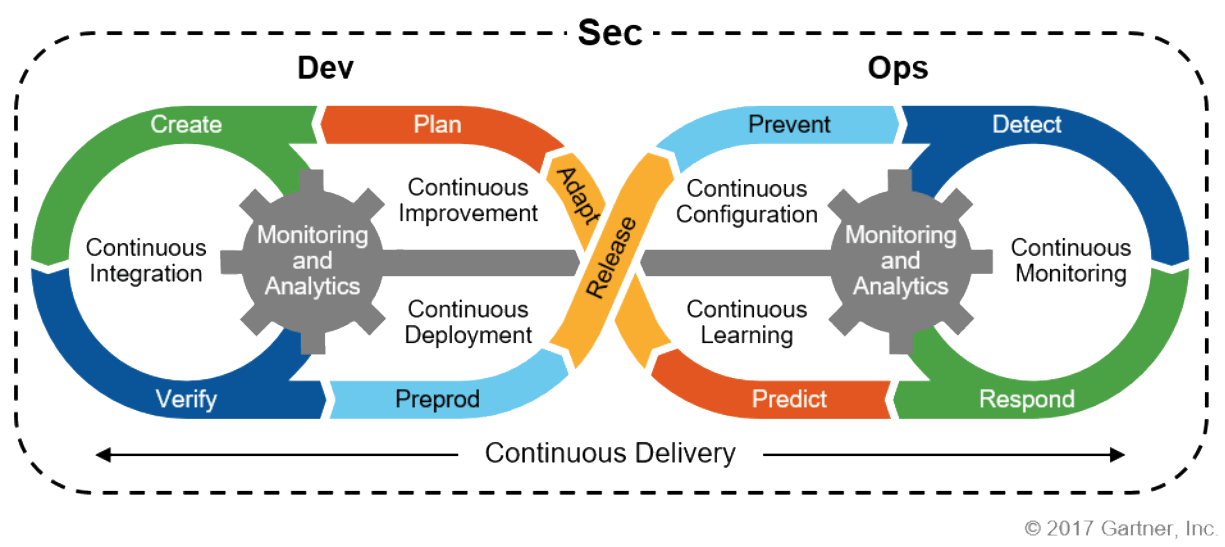
\includegraphics[height=120pt]{appsec cycle}
    \caption{AppSec Cycle}
    \label{fig:Figura2logo.1}
\end{figure}

\clearpage

\section{Cloud security}
\cite{cybersecurityguide}
\normalsize{Cloud security ou segurança da cloud refere-se a um conjunto de políticas, procedimentos tecnológicos, serviços e soluções designados para suportar de forma segura a nossa cloud (“nuvem de armazenamento”).
Quer seja operando de forma pública, privada ou até híbrida a segurança da nossa cloud é bastante importante e por isso devemos criar e manter estratégias preventivas e ações para combater as ameaças as nossas informações e dados presentes.\\
Como todos sabemos, uma cloud apenas é de confiança e deve ser usada se garantir aos seus utilizadores a segurança máxima, pois aí a segurança dos seus dados não depende apenas dos proprietários da rede, mas da companhia que fornece esses serviços. A principal vantagem da cloud é ser acessível a través de todos os nossos dispositivos diretamente sem a necessidade de ter armazenado nada no nosso dispositivo e por isso consideramos a segurança das clouds ainda mais complexa que a de uma simples rede interna. 
As ameaças às clouds são em muito semelhantes às das típicas redes internas, ter um novo ponto de acesso à nossa rede com tudo armazenado e sem ocupar espaço no nosso armazenamento local é muito bom para nós, mas também para os hackers que com isto, têm um novo ponto onde podem explorar vulnerabilidades e falhas de segurança. Porém isto não é uma tarefa fácil uma vez que maior parte dos fornecedores destes serviços de cloud garantem uma boa segurança infraestrutural.\\
Outro risco é o facto de qualquer um poder criar uma cloud e tentar enviar scripts para os servidores fornecedores da cloud de forma a tentar explorar falhas de segurança atingindo assim as várias empresas que dependem desse fornecedor da cloud.
Sendo um serviço disponível a todos é algo bom, mas isto quer dizer que todos somos responsáveis sobre o que introduzimos na cloud assim também é importante termos em atenção a própria segurança da cloud se queremos algo seguro não devemos trazer os riscos e ameaças até a nossa cloud.
E sendo um serviço disponível online é importante ter em atenção o possível risco de \ac{DDoS} dos quais devemos ter uma proteção e a possibilidade de os bloquear.}


\section{End-user education}
\cite{cyberdefensemagazine}
\normalsize{Muitas empresas preocupam em gastar grande quantidade de dinheiro em software, hardware e serviços para ajudar a prevenir ataques cibernéticos, mas acabam por se esquecer do treinamento do seu End-user, que geralmente é o elo mais fraco quando se fala em segurança cibernética e então os invasores aproveitam-se disso. Isto acontece não por culpa própria do End-user, mas sim por causa da falta de conhecimento perante estas ameaças cibernéticas. Esta técnica de engenharia social para enganar os funcionários de uma dada empresa, de forma a obter várias informações confidenciais, tem como nome phishing. O phishing é uma técnica tão popular para espalhar ransomware, isto é, um malware que bloqueia o acesso ao sistema infetado e que cobra um resgate em dinheiro para retirar o bloqueio, que também torna praticamente impossível o rastreamento do criminoso que pode vir a receber a quantia. \\

Para evitar que os end-users sejam enganados, a empresa deve de fazer um programa de treinamento de segurança, mas as informações devem ser dadas a um nível técnico que todos possam perceber, pois caso sejam muito elaboradas e ‘secantes’ eles perderão o interesse em aprender. Mesmo assim, há várias empresas que acham uma perda de tempo realizar tais programas, visto que pensam que seus funcionários não têm qualquer interesse ou não suficientemente inteligentes para perceber o conteúdo. Mas isto é uma maneira errada de pensar, porque eles estarão a ensiná-los e com isso a aperfeiçoar os seus conhecimentos, que lhe podem vir a ser úteis em casa, como ensinar aos filhos/família ou até a evitar catástrofes em suas residências. Existe vários sites, como o SANS, que contêm informações para ajudar uma empresa a organizar tais programas. \\

	Como podemos ver, a cibersegurança é muito importante porque protege todas as categorias de dados contra tentativas de roubo e danos. Como dados confidenciais, informações de identificação pessoal (PII), informações protegidas de saúde (PHI), informações pessoais, propriedade intelectual, informações governamentais e do setor. Esses programas de defesa cibernética é do interesse de todos, pois só traz aspetos positivos. Caso não tenhamos nenhum desses programas de cibersegurança, estaremos mais abertos a entrada de várias ameaças, tornando-nos um alvo ‘irresistível’ para os cibercriminosos e sermos incapazes de nos defender.
\begin{figure}[hp]
    \center 
    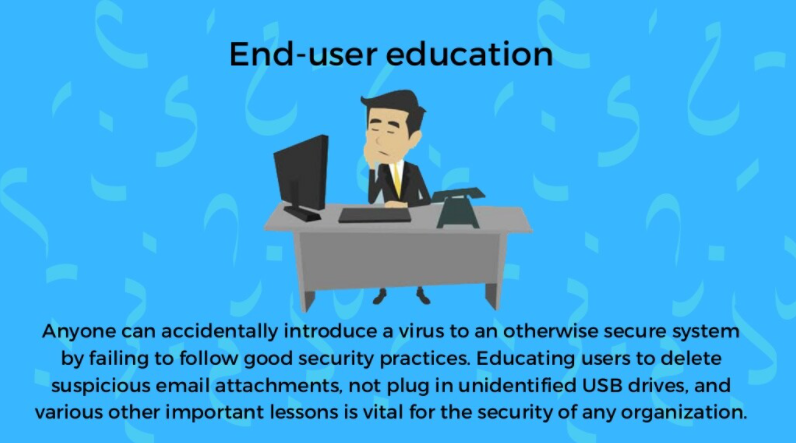
\includegraphics[height=150pt]{end-usereducation.PNG}
    \caption{End-User Education}
\label{fig:Figura3logo.1}
\end{figure}
	}


\clearpage

 \section{Boas práticas de cibersegurança}


De seguida e de forma a dar a conhecer a grande importância de manter as nossas informações e dados seguros vamos apresentar as principais praticas de cibersegurança:
\begin{enumerate}

\item Manter o software atualizado: As companhias de software tipicamente apresentam as atualizações de forma a trazer novas funcionalidades, corrigir bugs e melhorar a segurança.
\item Evitar abrir emails suspeitos- Se um email parecer suspeito, não o devemos abrir pois poderá ser malicioso, uma prática bastante usada por hackers é enviar emails imitando outra pessoa ou companhia de forma a obter uma entrada para os nossos dispositivos ou informação.
\item Manter o Hardware atualizado: Tal como é importante manter o software atualizado, devemos também tentar hardware mais recente que garantirá a possibilidade de ter o software mais recente e também uma velocidade de resposta maior aos ataques.
\item Usar uma forma segura de partilhar ficheiros como por exemplo as VPNs ou os serviços de cloud(referencias).
\item Antivírus e Antimalware(referencia): Como referidos estes softwares são capazes de nos garantir uma melhor segurança quando conectados à internet e a analise de ficheiros que possam conter software malicioso.
\item	É importante também ter em atenção os links que abrimos, pois estes poderão estar a redirecionar-nos a sites maliciosos ou diretamente a recolher informação nossa. Por isso é importante verificar os links em que clicamos.
\item Ter em atenção as nossas passwords, se a password existe é para proteger algo importante e por isso devemos criar uma password forte e segura de forma a garantir que estamos realmente protegidos.
\item Evitar usar redes publicas é também muito importante, pois qualquer pessoa tem acesso a essa rede e à informação que partilhamos. Quando não for possível evitar, devemos tentar usar uma VPN (referencia).
\item É também importante criar cópias de segurança e backups de segurança, de forma a termos sempre forma de aceder a nossa informação caso exista alguma falha de segurança.
\item Uma das práticas que tem se tornado cada vez mais popular consiste na contratação de um “White hat hacker”(ref), nem todos os hackers têm intenções más e a contratação de um hacker para testar a nossa segurança é uma das maneiras mais eficazes de testar a nossa segurança.
\end{enumerate} 
\section{Sinais de que podemos ter sido atacados}

\normalsize{Infelizmente a cibersegurança pode falhar em qualquer tipo de software, e a maioria dessas falhas devem-se a erros feitos pelo/por um utilizador (através do phishing). Os sinais mais comuns de acidentes cibernéticos são: 
\begin{itemize}
    \item   \textbf{Modificação de arquivos : } Caso alguns arquivos importantes comecem a alterarem de pastas ou até a se alterarem, como remover, substituir ou alterar, isto pode indicar que existe um cibercriminoso acessando o seu sistema sem qualquer permissão;
    
    \item   \textbf{Rede ou conexão com a Internet lentas : } Além do tópico anterior, se o dispositivo esteja mais lento do que o normal, também pode indicar tentativas de hacking contra o seu sistema, que pode levar ao cabo de um aumento no tráfego de rede;
    
    \item   \textbf{Emails de phishing : } Um ataque de phishing é quando alguém tenta convencer uma certa pessoa a clicar num link que mandou de maneira que consiga informações pessoais/confidenciais, ou até sem link! De forma a conseguirem abranger uma grande quantidade de pessoas em apenas ‘um click’, eles criam botnets (botnets são uma certa quantidade de dispositivos conectados á Internet, que vão executando um ou mais bots, sendo usada para ataques de \ac{DDoS}, enviar spam e roubar dados). Ao clicar nesses links, os bots conseguem captar informações confidenciais sem o conhecimento do ‘sofredor do ataque’. Com as informações de alguém, um cibercriminoso consegue fazer várias ações, como usar fazer passar-se por alguma pessoa ou até mesmo usar a sua identidade para acessar outras contas confidenciais (como contatos pessoais e bancários). Este tipo de ataques são das maiores ameaças digitais. Estes ataques costumam enganar várias pessoas devido a marcas que as pessoas confiam, por exemplo, á pessoas que recebem emails falsos dos \ac{CTT}, que ás vezes comentam ‘falha na entrega do produto com a referência: ***** ‘ ou ‘erro na entrega por favor verificar correio postal’ e ao clicar no link aparece para introduzir o cartão de débito, devido ao novo envio da sua encomenda e o preço a pagar que por vezes pode ser baixo, mas os cibercriminosos fazem de propósito esses valores baixos para enganar, de forma a que as pessoas pensem ‘Oh este valor é muito baixo para ser um hacker que me quer roubar, o que ele consegue fazer só com esta quantia de dinheiro?’, e esquecem que estão a introduzir as informações confidenciais dos seus cartões de débito, o que na realidade as fará ‘gastar mais dinheiro’. Para evitar tais acontecimentos devemos sempre ver o correio eletrónico e compará-lo ao original dessa marca, revisando a ortografia e até a gramática da palavra e garantido que o e-mail pareça legítimo;
    
    \item   \textbf{Adulteração de dispositivo : } Se o dispositivo desligue do nada e volte ao normal, isto pode indicar uma tentativa de entrada não autorizada, logo deve de ser realizada uma verificação antes de acessar informações confidenciais;
    
    \item   \textbf{Atividade incomum : } Também, se acontecer coisas estranhas relacionadas à senha, como um link para alteração da senha, e se o email não por da plataforma em que se encontra essa senha/email, é um sinal óbvio que sofreu um ataque cibernético. De forma a lidar com esse problema, devemos alterar a senha imediatamente e aproveitar para torná-la mais ‘eficaz’, isto é, acrescentar maiúsculas, minúsculas, números e caracteres (ou usar um gerenciador de senhas confiável (o que não pode ser também muito aconselhado));
    
    \item   \textbf{Tentativas de falha de login : } se não conseguir efetuar login normalmente em sua conta, isto pode ser um sinal de comprometimento, caso aconteça, devemos redefinir a senha e realizar login novamente, se falhar, devemos imediatamente contactar o serviço, onde estamos a realizar o login, e alertá-los da probabilidade da nossa conta ter sido comprometida á um cibercriminoso
	\end{itemize}
\chapter{Conclusões}
\label{chap.conclusao}
A partir da resolução do trabalho concluimos que com o aumento crescente e exponencial da Internet geograficamente, no número de seus utilizadores e nos serviços disponibilizados, também fez com que aparecessem vários desafios/ameaças no ciberespaço.\\ Para que isto fosse/seja evitado, foi/é necessário também o crescimento da área da cibersegurança para evitar várias catástrofes em cloud, aplicativos, infraestruturas, informações confidenciais....\\ Qualquer pessoa pode contribuir para a diminuição destas ameaças cibercriminosas, no modo em que cada uma se informe melhor sobre tais ameaças, evitando pôr a sua empresa em risco e a sua habitação.Simples ações podem tronar-se impactantes!

\begin{figure}[hp]
    \center 
    
\includegraphics[height=200pt]{ciberseguranca-2.jpeg}
    \caption{Pesquise, informe-se, aprende!}
    \label{fig:Figura4logo.1}
\end{figure}


\chapter*{Contribuições dos autores}

As contribuições dos autores para este documento foram:

\begin{description}
	\item[\ac{MR}] - Introdução, O que é a cibersegurança?,Network Security,Cloud Security,Boas praticas de Cibersegurança, bibliografia, pesquisa de informação;
	\item[\ac{HC}] - Resumo,Critical Infrastructural Security,Application Security,End-User Education, Sinais de que podemos ter sido atacados,Conclusões,pesquisa de informação;
\end{description}

Como tal, e também com base nas estatísticas das revisões do code.ua, pode-se afirmar que a percentagem de contribuição de cada um foi:

\begin{description}
	\item[\ac{MR}] - 50\%
	\item[\ac{HC}] - 50\%
\end{description}
%%%%%%%%%%%%%%%%%%%%%%%%%%%%%%%%%

\chapter*{Acrónimos}
\begin{acronym}
\acro{ua}[UA]{Universidade de Aveiro}
\acro{CIP}{Critical Infrastructure security}
\acro{EPCIP}{European Programme for Critical Infrastructure Protection}
\acro{EUA}{Estados Unidos da América}
\acro{ISO/IEC}{Internatonal Organization for Standardization/Interantional Electrotechnical Commission}
\acro{DAST/SAST} {Dynamic Application Security Testing/Static Application Security Testing}
\acro{SANS}{System Administration,Network and Security}
\acro{PII}{Personally Identifiable Information}
\acro{PHI}{Protected Health Information}
\acro{DDOS}{Distributed Denial of Services}
\acro{CTT}{Correios de Portugal}
\acro{HTTP}{Hypertext Transfer Protocol}
\acro{VPN}{Virtual Privacy Network}
\acro{DNS}{Domain Name System}
\acro{MR}{Miguel Reis}
\acro{HC}{Henrique Coelho}
\end{acronym}


%%%%%%%%%%%%%%%%%%%%%%%%%%%%%%%%%
\printbibliography

\end{document}
